\documentclass{beamer}
%\documentclass[xcolor=dvipsnames]{beamer}
\usepackage[spanish]{babel}
\usepackage[utf8]{inputenc}
\usepackage{graphicx}
\usepackage{epstopdf}

\newcommand{\beamer}{\textsc{beamer}}
\newtheorem{definicion}{Definición}
\newtheorem{ejemplo}{Ejemplo}

%%%%%%%%%%%%%%%%%%%%%%%%%%%%%%%%%%%%%%%%%%%%%%%%%%%%%%%%%%%%%%%%%%%%%%%%%%%%%%%
\title[Integración: Simpson]{Integración: Simpson\\$f(x)=x^{2}\ cos\ x,\ x \in [1,3]$}
\author[Adrián R. / Roberto C.]{Adrián R. Mendióroz Morales\\Roberto C. Palenzuela Criado}
\institute[ULL]{Universidad de La Laguna}
\date[13-05-13]{13 de mayo de 2013}
%%%%%%%%%%%%%%%%%%%%%%%%%%%%%%%%%%%%%%%%%%%%%%%%%%%%%%%%%%%%%%%%%%%%%%%%%%%%%%%

\usetheme{Madrid}

%%%%%%%%%%%%%%%%%%%%%%%%%%%%%%%%%%%%%%%%%%%%%%%%%%%%%%%%%%%%%%%%%%%%%%%%%%%%%%%
\definecolor{pantone254}{RGB}{122,59,122}
\definecolor{pantone3015}{RGB}{0,88,147}
\definecolor{pantone432}{RGB}{56,61,66}
\setbeamercolor*{palette primary}{use=structure,fg=white,bg=pantone254}
\setbeamercolor*{palette secondary}{use=structure,fg=white,bg=pantone3015}
\setbeamercolor*{palette tertiary}{use=structure,fg=white,bg=pantone432}
\setbeamercolor*{palette sidebar primary}{use=structure,fg=pantone254}
\setbeamercolor*{palette sidebar tertiary}{use=structure,fg=pantone3015}
\setbeamercolor*{block title}{bg=pantone3015,fg=white}
\setbeamercolor*{alerted text}{fg=pantone432}
\setbeamercolor*{item projected}{fg=pantone254}
\setbeamercolor*{section in toc shaded}{use=structure,fg=structure.fg}
\setbeamercolor*{section in toc}{fg=pantone3015}
\setbeamercolor*{subsection in toc shaded}{fg=pantone3015}
\setbeamercolor*{subsection in toc}{fg=pantone432}

%%%%%%%%%%%%%%%%%%%%%%%%%%%%%%%%%%%%%%%%%%%%%%%%%%%%%%%%%%%%%%%%%%%%%%%%%%%%%%%
\begin{document}
%++++++++++++++++++++++++++++++++++++++++++++++++++++++++++++++++++++++++++++++  
\begin{frame}

  
\includegraphics[width=0.15\textwidth]{img/ullesc.eps}
  \hspace*{7.5cm}
  
\includegraphics[width=0.16\textwidth]{img/fmatesc.eps}
  \titlepage

  \begin{scriptsize}
    \begin{center}
     Facultad de Matemáticas \\
     Universidad de La Laguna
    \end{center}
  \end{scriptsize}

\end{frame}
%++++++++++++++++++++++++++++++++++++++++++++++++++++++++++++++++++++++++++++++  

%++++++++++++++++++++++++++++++++++++++++++++++++++++++++++++++++++++++++++++++  
\begin{frame}
  \frametitle{Índice}  
  \tableofcontents[pausesections]
\end{frame}
%++++++++++++++++++++++++++++++++++++++++++++++++++++++++++++++++++++++++++++++  

\section{Motivación y Objetivos}

%++++++++++++++++++++++++++++++++++++++++++++++++++++++++++++++++++++++++++++++  
\begin{frame}

  \frametitle{Motivación}

  \begin{block}{}
    Aprender a aplicar conocimientos matemáticos de forma profesional en la 
    elaboración y defensa de argumentos y en la resolución de problemas.
  \end{block}

\end{frame}
%++++++++++++++++++++++++++++++++++++++++++++++++++++++++++++++++++++++++++++++  

%++++++++++++++++++++++++++++++++++++++++++++++++++++++++++++++++++++++++++++++  
\begin{frame}

  \frametitle{Objetivos}

  \begin{block}{}
    \begin{itemize}
      \item Investigar el método numérico de la Regla de Simpson. 
      \item Aplicar la Regla de Simpson a la función $f(x)=x^{2}\ cos\ x$, en el intervalo $[1,3]$.
    \end{itemize}
  \end{block}

\end{frame}
%++++++++++++++++++++++++++++++++++++++++++++++++++++++++++++++++++++++++++++++  

\section{Fundamentos Teóricos}

%++++++++++++++++++++++++++++++++++++++++++++++++++++++++++++++++++++++++++++++
\begin{frame}

  \frametitle{Fundamentos Teóricos}
  
  La necesidad de aproximar numéricamente el valor de una integral surge fundamentalmente por dos motivos:
  \begin{itemize}
    \item La dificultad o imposibilidad en el cálculo de una primitiva.
    \item La función a integrar sólo se conoce por una tabla de valores.
  \end{itemize}
  El problema básico considerado por la integración numérica es calcular una solución
  aproximada a la integral definida:
  \[\int_{a}^{b} f(x)\ \text{d}x \]
  Los métodos más comunes de integración numérica son:
  \begin{itemize}
    \item La regla del Trapecio.
    \item La regla de Simpson.
  \end{itemize}
  
\end{frame}
%+++++++++++++++++++++++++++++++++++++++++++++++++++++++++++++++++++++++++++++++++++
\begin{frame}
  
  \frametitle{Fundamentos Teóricos}
  
  \begin{block}{Regla de Simpson}
    Se desea aproximar la integral:
    \[ I = \int_{a}^{b} f(x) \text{d}x \]
    \begin{center}
      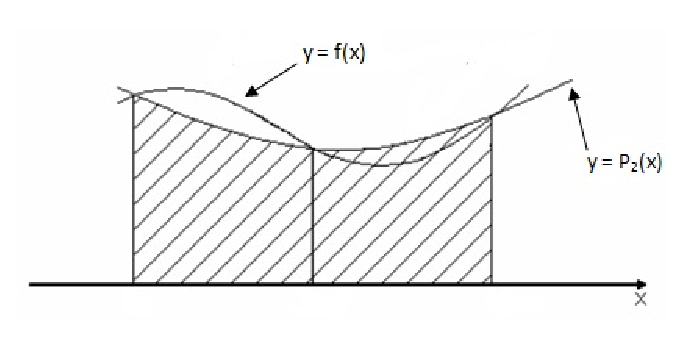
\includegraphics[width=0.50\textwidth]{img/Grafica_Simpson.eps}
    \end{center}  
  \end{block}
 
\end{frame}
%+++++++++++++++++++++++++++++++++++++++++++++++++++++++++++++++++++++++++++++++++++
\begin{frame}

  \frametitle{Fundamentos Teóricos}
  
  \begin{block}{Regla de Simpson}
    \[ \int_{a}^{b} f(x) \text{d}x \approx \frac{b-a}{6}\left[f(a) + 4f\left(\frac{a+b}{2}\right) + f(b)\right] \]
    \[\text{Error asociado: } -\frac{1}{90}(b-a)^5f^{(4)}(\xi), \quad \xi \in (a,b)\]
  \end{block}

\end{frame}
%++++++++++++++++++++++++++++++++++++++++++++++++++++++++++++++++++++++++++++++++++++
\begin{frame}

  \frametitle{Fundamentos Teóricos}
  
  \begin{block}{Regla de Simpson Compuesta}
    \[ \int_{a}^{b}f(x) \text{d}x \approx \frac{h}{3}\left[f(x_0) + 2\sum_{j=1}^{\frac{n}{2}-1} f(x_{2j}) + 
    4\sum_{j=1}^{\frac{n}{2}} f(x_{2j-1}) + f(x_n)\right] \]
    \[\text{Error asociado: }-\frac{1}{180}(b-a)h^4f^{(4)}(\xi), \quad \xi \in (a,b) \]
  \end{block}

\end{frame}
%++++++++++++++++++++++++++++++++++++++++++++++++++++++++++++++++++++++++++++++  

\section{Procedimiento experimental}

%++++++++++++++++++++++++++++++++++++++++++++++++++++++++++++++++++++++++++++++  

\subsection{Descripción de los experimentos}

%++++++++++++++++++++++++++++++++++++++++++++++++++++++++++++++++++++++++++++++  
\begin{frame}

  \frametitle{Procedimiento experimental}

  \begin{block}{Descripci\'on de los experimentos}
    \begin{itemize}
      \item <1-> Representación gráfica de la función.
      \pause
      \item <2-> Cálculo del valor exacto de la integral definida.
      \pause  
      \item <3-> Comparación gráfica.
      \pause
      \item <4-> Aproximación por la Regla de Simpson.
      \pause
      \item <5-> Aproximación por la Regla de Simpson compuesta.
    \end{itemize}
  \end{block}

\end{frame}
%+++++++++++++++++++++++++++++++++++++++++++++++++++++++++++++++++++++++++++++++
\begin{frame}

  \frametitle{Descripción de los experimentos}
  
  \begin{block}{Representación gráfica de la función}
    \begin{center}
      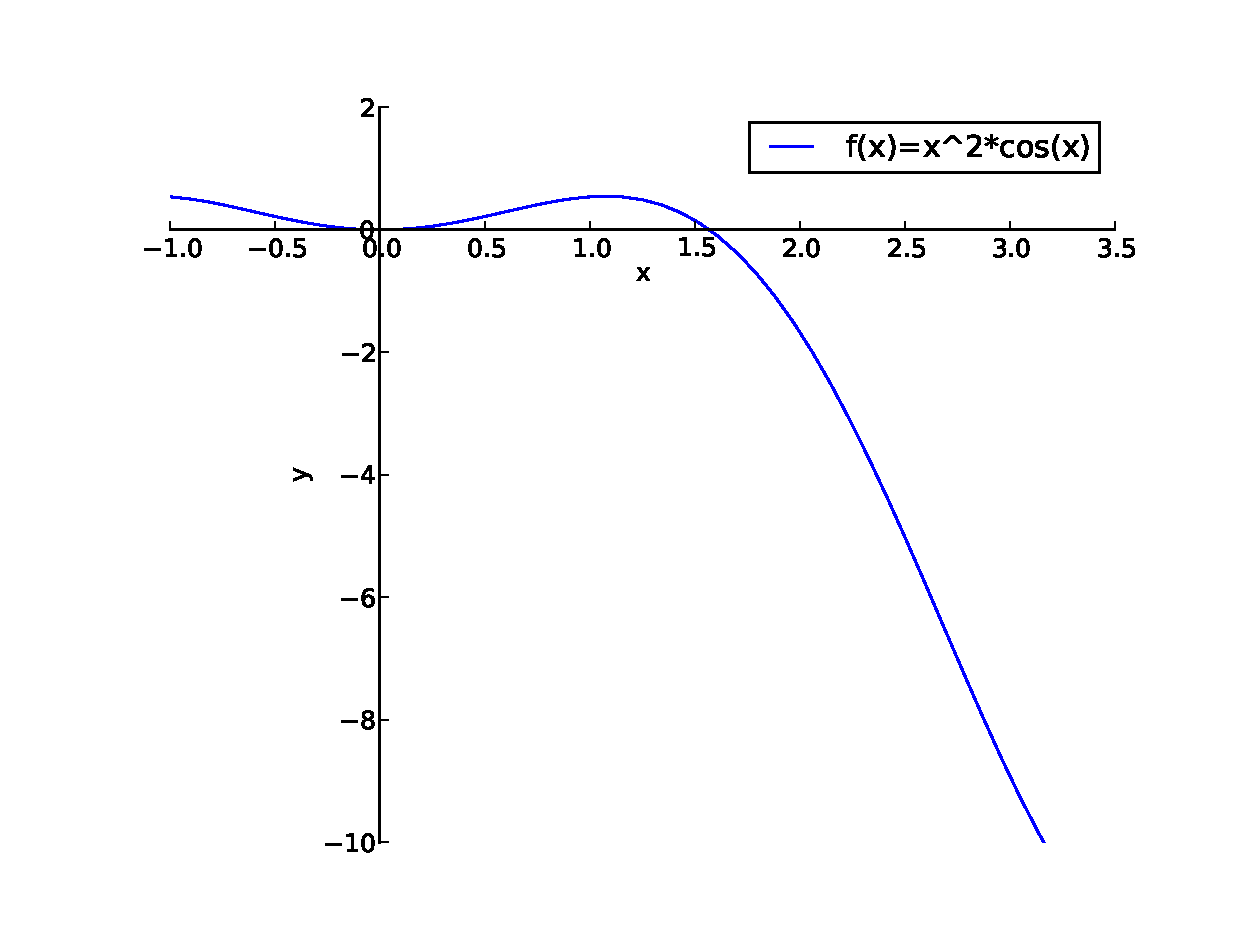
\includegraphics[width=0.75\textwidth]{img/grafica1.eps}
    \end{center}
  \end{block}

\end{frame}
%+++++++++++++++++++++++++++++++++++++++++++++++++++++++++++++++++++++++++++++++
\begin{frame}

  \frametitle{Descripción de los experimentos}
  
  \begin{block}{Cálculo del valor exacto de la integral definida}
    \begin{itemize}[<+->]
     \item \[ \int_{1}^{3} x^2\ cos\ x\ \text{d}x  \]
     \item \[ \int x^2\ cos\ x\ \text{d}x = 2x cos\ x + (x^2 -2)sen\ x +C=F(x)+C\]
     \item \[ \int_{1}^{3} x^2\ cos\ x\ \text{d}x = F(3)-F(1)\]
    \end{itemize}   
  \end{block}

\end{frame}
%+++++++++++++++++++++++++++++++++++++++++++++++++++++++++++++++++++++++++++++++
\begin{frame}

  \frametitle{Descripción de los experimentos}
  
  \begin{block}{Comparación Gráfica}
    \begin{center}
      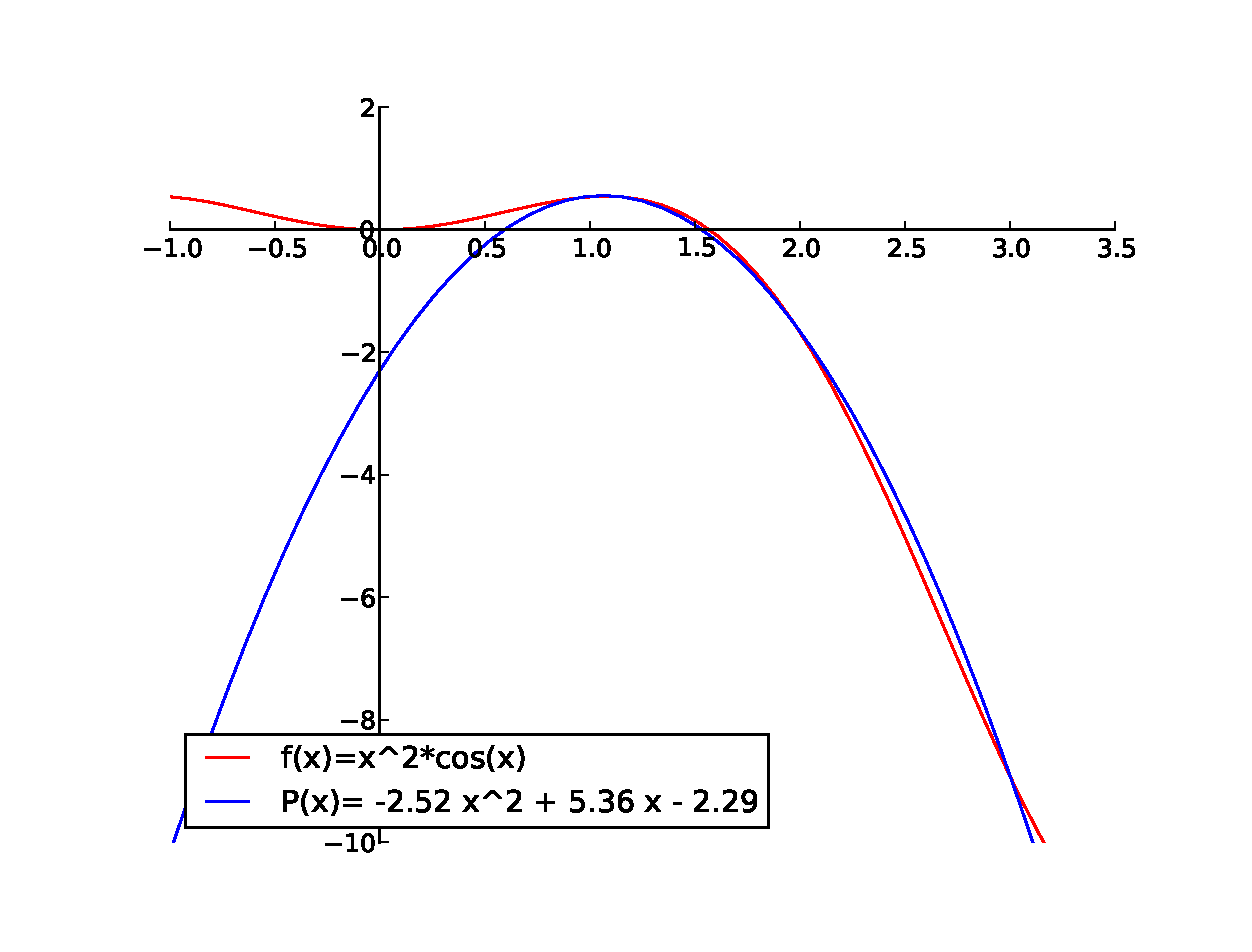
\includegraphics[width=0.75\textwidth]{img/grafica2.eps}
    \end{center}
  \end{block}
 
\end{frame}
%+++++++++++++++++++++++++++++++++++++++++++++++++++++++++++++++++++++++++++++++
\begin{frame}[fragile]

  \frametitle{Procedimiento experimental}
  
  \begin{block}{Aproximación por la regla de Simpson}
    Función:
      \begin{center}
        \begin{footnotesize}
          \begin{verbatim}
def regla_simpson(f,a,b):
  return (b-a)/6.0*(f(a)+4*f((a+b)/2.0)+f(b))
          \end{verbatim}
        \end{footnotesize}
      \end{center}
    Programa Principal:
      \begin{center}
        \begin{footnotesize}
          \begin{verbatim}
from simpson import regla_simpson
from math import *
F=(2*3*cos(3)+(3**2-2)*sin(3))-(2*1*cos(1)+(1**2-2)*sin(1))
print '\nValor real= ',F
aprox=regla_simpson(lambda x:(x**2*cos(x)),1,3)
print '\nAproximacion por la regla de Simpson: ',aprox
          \end{verbatim}
        \end{footnotesize}
      \end{center}
  \end{block}
  
\end{frame}
%+++++++++++++++++++++++++++++++++++++++++++++++++++++++++++++++++++++++++++++
\begin{frame}[fragile]

  \frametitle{Procedimiento experimental}
  
  \begin{block}{Aproximación por la regla de Simpson compuesta}
    Función:
    \begin{center}
      \begin{footnotesize}
        \begin{verbatim}
def regla_simpson_compuesta(f,a,b,n):
  h=(b-a)/float(n)
  aprox=0
  for l in range(0,n):
    aprox+=regla_simpson(lambda x:(x**2*cos(x)),
    a+l*h,a+(l+1)*h)
  return aprox
        \end{verbatim}
      \end{footnotesize}
    \end{center}
  \end{block}
  
\end{frame}
%++++++++++++++++++++++++++++++++++++++++++++++++++++++++++++++++++++++++++++++  
\begin{frame}[fragile]

  \frametitle{Procedimiento experimental}
  
  \begin{block}{Aproximación por la regla de Simpson compuesta}
    Programa Principal:
    \begin{center}
      \begin{footnotesize}
        \begin{verbatim}
from simpson import regla_simpson_compuesta
from math import *
F=(2*3*cos(3)+(3**2-2)*sin(3))-(2*1*cos(1)+(1**2-2)*sin(1))
print 'Valor real= ',F
print 'Aproximacion por la regla de Simpson compuesta: '
print '%25s %15s %15s %15s' % ('Numero de subintervalos',
'Aproximacion','Error absoluto','Error relativo')
n=[2,6,10,50,100]
aprox=0
i=0
for l in n:
  aprox=regla_simpson_compuesta(lambda x:(x**2*cos(x)),1,3,l)
  print '%16d %24.10f %15.10f %15.10f' %(n[i],aprox,abs(F-aprox),
  abs(F-aprox)/abs(F))
  i=i+1
        \end{verbatim}
      \end{footnotesize}
    \end{center}
  \end{block}
  
\end{frame}
%++++++++++++++++++++++++++++++++++++++++++++++++++++++++++++++++++++++++++++++
\subsection{Descripción del material}

%++++++++++++++++++++++++++++++++++++++++++++++++++++++++++++++++++++++++++++++  
\begin{frame}

  \frametitle{Descripción del material}
  
  \begin{block}{Hardware}
    \begin{itemize}
      \item CPU type: Intel(R) Atom(TM) CPU N270   @ 1.60GHz
      \item CPU speed: 800.000Hz
      \item Cache size: 512 KB
    \end{itemize}
  \end{block}

  \begin{block}{Software}
    En cuanto al sistema operativo, se ha utilizado ``Linux-3.2.0-39-generic-i686-with-Ubuntu-12.04-precise''.
    Los ficheros en lenguaje Python fueron realizados con el editor de textos avanzado para KDE ``Kate''.
  \end{block}

\end{frame}
%++++++++++++++++++++++++++++++++++++++++++++++++++++++++++++++++++++++++++++++  

\subsection{Resultados obtenidos}

%++++++++++++++++++++++++++++++++++++++++++++++++++++++++++++++++++++++++++++++  
\begin{frame}
  
  \frametitle{Resultados Obtenidos}
  
  %--------------------------------------------------------------------------
\begin{table}[h]
\begin{center}
\begin{tabular}{|c|c|c|c|} \hline 
\textbf{Valor exacto} & \textbf{Aproximacion} & \textbf{Error absoluto} & \textbf{Error relativo}\\ 
\hline
-5.19124855011 & -5.0093265161 & 0.181922034015 & 0.0350439845558
\\
\hline
\end{tabular}
\end{center}
\caption{Aproximacion y error de la regla de Simpson}
\label{tab:1}
\end{table}


  %--------------------------------------------------------------------------
\begin{table}[h]
  \begin{center}
    \begin{tabular}{|c|c|c|c|c|} \hline 
      \textbf{N\'umero de subintervalos} & \textbf{Aproximaci\'on} & \textbf{Error absoluto} & \textbf{Error relativo}\\ 
      \hline
      2 & -5.1817934049 & 0.0094551452 & 0.0018213625
      \\
      \hline
      6 & -5.1911377092 & 0.0001108409 & 0.0000213515
      \\
      \hline
      10 & -5.1912342437 & 0.0000143064 & 0.0000027559
      \\
      \hline
      50 & -5.1912485273 & 0.0000000228 & 0.0000000044
      \\
      \hline
      100 & -5.1912485487 & 0.0000000014 & 0.0000000003
      \\
      \hline
    \end{tabular}
  \end{center}
  \caption{Aproximaci\'on y error de la regla de Simpson compuesta}
  \label{tab:2}
\end{table}



\end{frame}
%++++++++++++++++++++++++++++++++++++++++++++++++++++++++++++++++++++++++++++++  

\subsection{Análisis de los resultados}

%++++++++++++++++++++++++++++++++++++++++++++++++++++++++++++++++++++++++++++++  
\begin{frame}

  \frametitle{Análisis de los resultados}
  
  %--------------------------------------------------------------------------
\begin{table}[h]
  \begin{center}
    \begin{tabular}{|c|c|c|c|c|} \hline 
      \textbf{V. exacto} & \textbf{Aprox.} & \textbf{E. absoluto} & 
      \textbf{E. relativo} & \textbf{C. signific.}\\ 
      \hline
      -5.19124855 & -5.0093265 & 0.18192203 & 0.03504398 & 2
      \\
      \hline
    \end{tabular}
  \end{center}
  \caption{Aproximaci\'on y error de la regla de Simpson}
  \label{tab:3}
\end{table}


  %--------------------------------------------------------------------------
\begin{table}[H]
  \begin{center}
    \begin{tabular}{|c|c|c|c|c|} \hline 
      \textbf{N} & \textbf{Aproximaci\'on} & \textbf{E. absoluto} & \textbf{E. relativo} & \textbf{C. S.}\\ 
      \hline
      2 & -5.1817934049 & 0.0094551452 & 0.0018213625 & 3
      \\
      \hline
      6 & -5.1911377092 & 0.0001108409 & 0.0000213515 & 5
      \\
      \hline
      10 & -5.1912342437 & 0.0000143064 & 0.0000027559 & 6
      \\
      \hline
      50 & -5.1912485273 & 0.0000000228 & 0.0000000044 & 9
      \\
      \hline
      100 & -5.1912485487 & 0.0000000014 & 0.0000000003 & 10
      \\
      \hline
    \end{tabular}
  \end{center}
  \caption{Aproximaci\'on y error de la regla de Simpson compuesta}
  \label{tab:4}
\end{table}



\end{frame}
%++++++++++++++++++++++++++++++++++++++++++++++++++++++++++++++++++++++++++++++  

\section{Conclusiones}

%++++++++++++++++++++++++++++++++++++++++++++++++++++++++++++++++++++++++++++++  
\begin{frame}
  
  \frametitle{Conclusiones}
  
  \begin{block}{}
    \begin{enumerate}[<+->]
      \item La integraci\'on num\'erica reduce el c\'alculo del valor de la integral 
      definida en el caso de funciones muy complejas, a simples operaciones aritm\'eticas.
      \item La Regla de Simpson simplifica el c\'alculo de una integral definida 
      compleja, aproximando su valor al de la integral de un polinomio de segundo 
      grado.
      \item La Regla de Simpson es m\'as precisa que otros m\'etodos como la Regla del 
      Trapecio a la hora de aproximar la integral.
      \item La Regla de Simpson proporciona aproximaciones exactas para polinomios 
      de grado menor o igual a tres.
    \end{enumerate}
 \end{block}

\end{frame}
%++++++++++++++++++++++++++++++++++++++++++++++++++++++++++++++++++++++++++++++++++++
\begin{frame}
  
  \frametitle{Conclusiones}
  
  \begin{block}{}
    \begin{enumerate}[<+->]
      \item La Regla de Simpson Compuesta proporciona aproximaciones m\'as precisas 
      que la Regla de Simpson.
      \item En la Regla de Simpson Compuesta, el error es inversamente proporcional 
      al n\'umero de subintervalos.
      \item En la Regla de Simpson Compuesta, el error es directamente proporcional 
      a la amplitud del intervalo.
    \end{enumerate}
 \end{block}

\end{frame}
%++++++++++++++++++++++++++++++++++++++++++++++++++++++++++++++++++++++++++++++  
\begin{frame}

  \frametitle{Bibliografía}
  
  \bibliographystyle{plain}
  \bibliography{bib/references.bib}
  \nocite{*}
  
\end{frame}
%++++++++++++++++++++++++++++++++++++++++++++++++++++++++++++++++++++++++++++++  
\end{document}
%%%%%%%%%%%%%%%%%%%%%%%%%%%%%%%%%%%%%%%%%%%%%%%%%%%%%%%%%%%%%%%%%%%%%%%%%%%%%%%%